\chapter{Reinforcement Learning Approach}\label{ch:reinforcement.learning.approach}

Several methods, in the scientific literature, focus on the use of Reinforcement Learning to attempt to explore environments that are \emph{unknown}. The objective is to determine the optimal set of actions to perform (the \emph{optimal policy}) in order to reach the objective.

In this work, a simple Reinforcement Learning algorithm working with drone's position has been tested to explore the subject.

\section{Formalization}

The agent considered is the drone and the environment, in the sense of Reinforcement Learning, is the environment in which the drone navigates (\eg{} Indoor Corridor).

The environment is considered as a two-dimensional grid. The position of the agent in the environment is given by its coordinates $i$ and $j$ in the grid. The latter represents the agent's state (noted $x$).

The agent interacts with its environment through a series of deterministic actions: move forward, move back, turn left and turn right. More formally, the action space $U$ is given by
\begin{equation}
    U = [(1, 0), (-1, 0), (0, 1), (0, -1)]
\end{equation}
When the agent interacts with its environment, it receives some \emph{rewards}: each displacement of the agent earns it a $-1$ reward, each obstacle taken earns it $-\infty$ and the objective reached earns it $100$. The agent's main goal is to maximize his total reward, \ie{} to reach the goal as quick as possible without hitting any obstacle.

\section{Optimal policy}

In order to calculate the optimal policy $\mu^*$ of the agent, a simple \emph{Q-learning} algorithm has been used. The optimal policy is given by
\begin{equation}
    \mu^*_N(x) = \arg\max_{u \in U}Q_N(x, u)
\end{equation}
where $x$ is the agent's state, $u$ is an action and $Q_N(x, u)$ is the state-action value.

The value $Q_N(x, u)$ can be calculated via the recurrence equation
\begin{equation}
    Q_{N}(x, u) = r(x, u) + \gamma \sum_{x^{\prime} \in X} p(x' \mid x, u) \max_{u^{\prime} \in U} Q_{N-1}\left(x^{\prime}, u^{\prime}\right), \quad \forall N \geq 1
\end{equation}
where $r(x, u)$ is the reward, $\gamma$ is a \emph{discount factor} reducing the importance of future rewards compared to immediate rewards and $p(x' \mid x, u)$ the transition probability of the \emph{Markov Decision Process} (MDP) corresponding to the domain. With a sufficient number of iterations $N$ (fixed so that the difference between the rewards of two optimal policies calculated is lower than a fixed threshold set to $\num{0.001}$), it is thus possible to calculate $Q_N$ and to deduce the optimal policy $\mu^*_N$.

This procedure was applied to the Indoor Corridor environment and to another complex environment. The obtained results are shown in Figure \ref{fig:C.reinforcement.learning.policies}.

\begin{figure}[H]
    \centering
    \begin{subfigure}{0.515\textwidth}
        \centering
        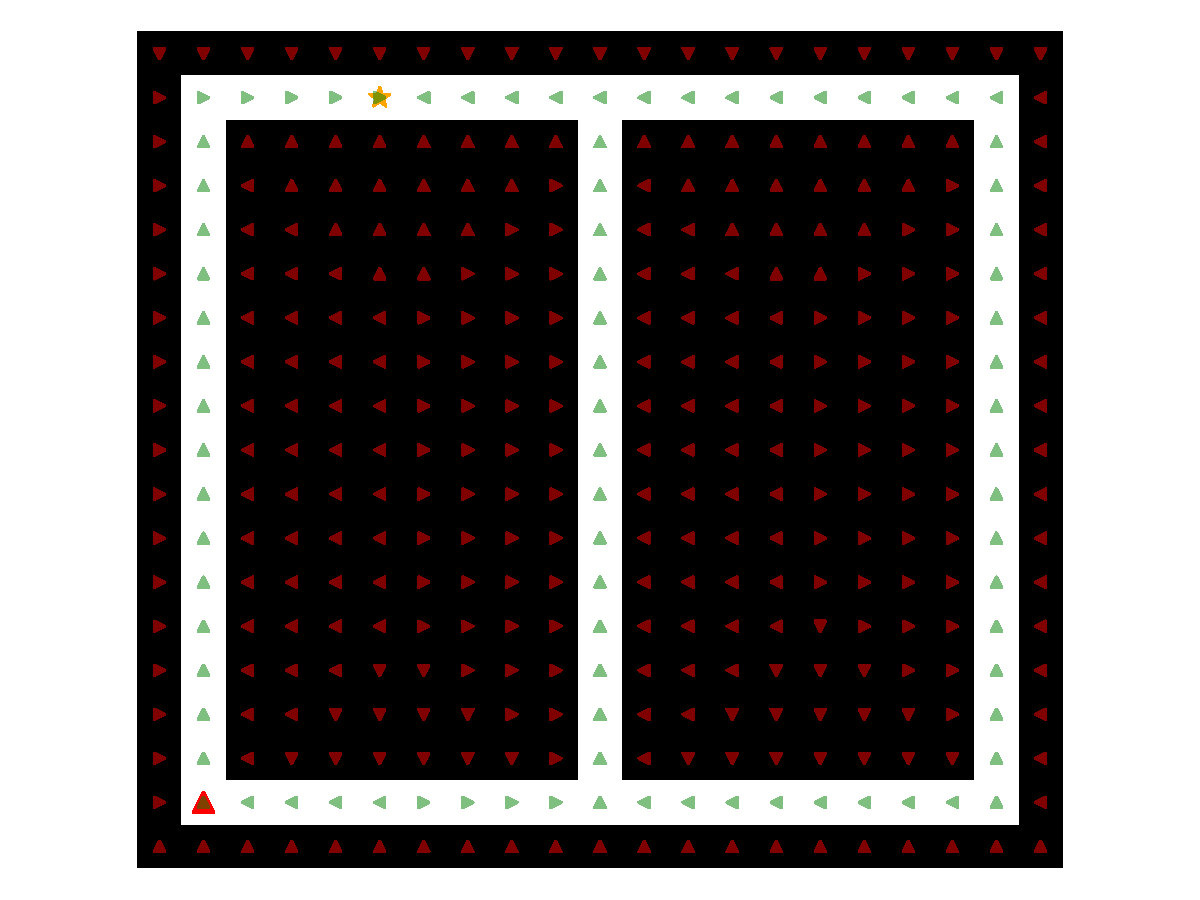
\includegraphics[width=\textwidth]{resources/pdf/C/indoor-corridor.pdf}
        \caption{Indoor Corridor}
    \end{subfigure}
    \hfill
    \begin{subfigure}{0.465\textwidth}
        \centering
        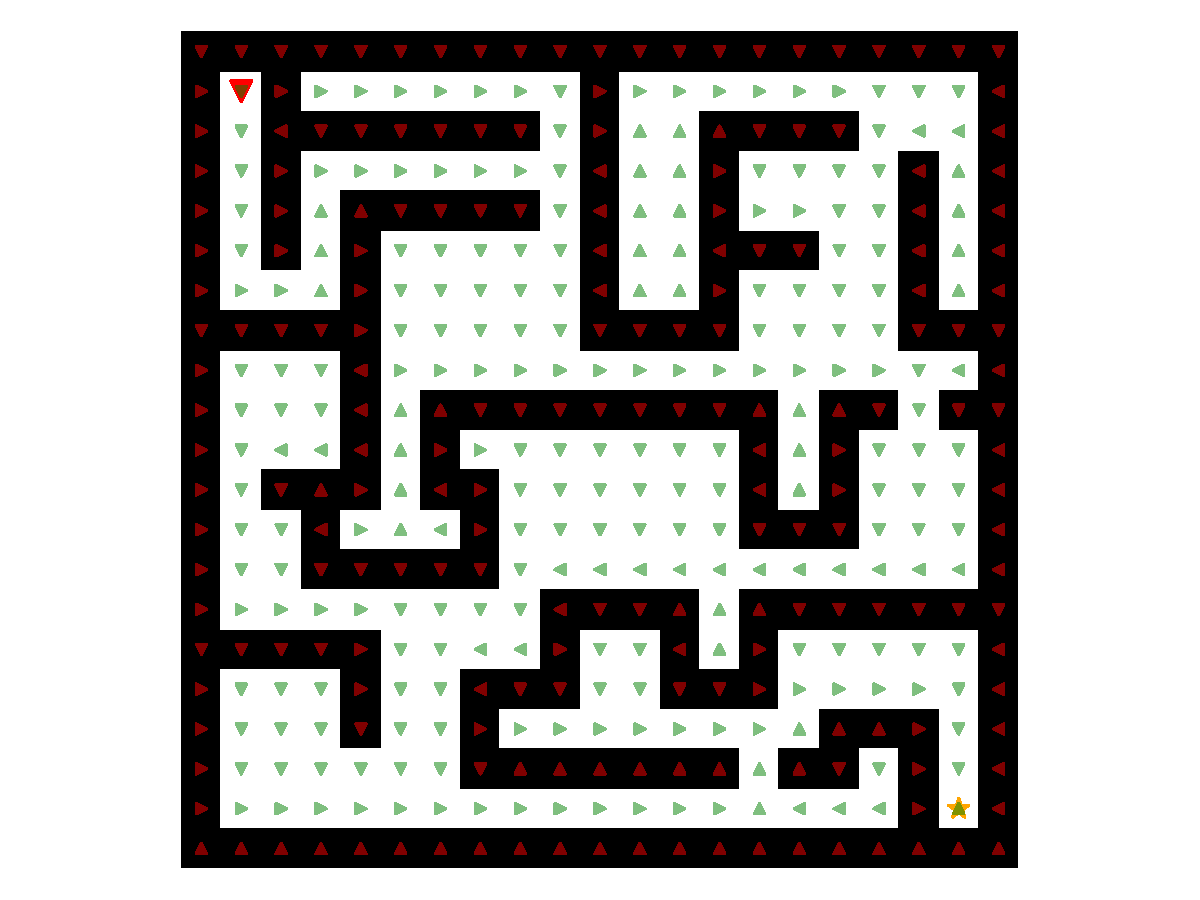
\includegraphics[width=\textwidth]{resources/pdf/C/complex.pdf}
        \caption{Complex}
    \end{subfigure}
    \caption{Optimal policies obtained via a simple Q-learning algorithm. The agent's position and orientation is represented by a red arrow. Its objective is represented by a yellow star. The action to be taken at each location in the environment is represented by a small arrow (green when the location is accessible and red when the location is inaccessible).}
    \label{fig:C.reinforcement.learning.policies}
\end{figure}

\section{Discussion}

The obtained results show that this procedure is effective in determining the optimal policy leading the drone from its starting point to the objective, in a totally unknown environment.

Although explored in several scientific papers (see Chapter \ref{ch:sota}), this procedure does not take into account the noisy displacements of the drone and the unanticipated dynamic obstacles in the environment. Moreover, the procedure experimented here considers that the environment is deterministic (whereas in real life it is stochastic) and totally observable. Also, this procedure works with the drone's position, which is not really realistic since this position can not be easily obtained in practice.

These simplifying assumptions allow us to obtain results showing that Reinforcement Learning can be a solution for autonomous navigation. However, more complex techniques need to be explored (\eg{} Deep Reinforcement Learning working with images) to hope to put this into practice in the real world, especially if we only have access to the drone's images (and not directly its position). Furthermore, since Reinforcement Learning works by trial and error, it is difficult to train a real drone in a real environment. It is then necessary to train a model on a simulator and apply it to the real world via Transfer Learning (see \cite{anwar2020autonomous}).

The further exploration of Reinforcement Learning methods, especially using only drone's images, will not be addressed in this work and are left for future work on the subject.
